\documentclass{article}

\usepackage{csc579}
\usepackage{amssymb,amsmath,amsthm}
\usepackage{tikz}
\usepackage{multicol}
\usepackage{enumitem}
\usepackage{gensymb}
\usepackage[T1]{fontenc}
\usepackage{inconsolata}
\usepackage{qtree}
\usepackage{pgfplots}
\usepackage{hyperref}

\thickmuskip=2mu

\begin{document}

\HWK{Project 1}{February 27, 2017}

\bigskip

\textbf{Task 1}
Let $N$ be the total number of customers that arrived to the system at the time the simulation ends (i.e., after the $C$-th customer completes service, $C ≤ N$). Let $X$ be the number of customers denied service (lost) at the time the simulation ends. Let us define the customer loss rate (CLR) as: $CLR =\frac{X}{N}$.

The CLR is one of the main metrics of interest in the M/M/1/K system. Let the queue capacity $K = 20$.
Plot the CLR against the value of $\rho$, for $\rho = 0.05$ to $\rho = 0.95$, in increments of 0.10. Submit two graphs: one for $C = 1,000$ and one for $C = 100,000$. Do you see any difference in the two plots? If so, can you explain the difference? If not, why do you think there is no difference? Explain your answer. Did you expect these
results before running the experiment?
\\
\medskip\\\texttt{
\\
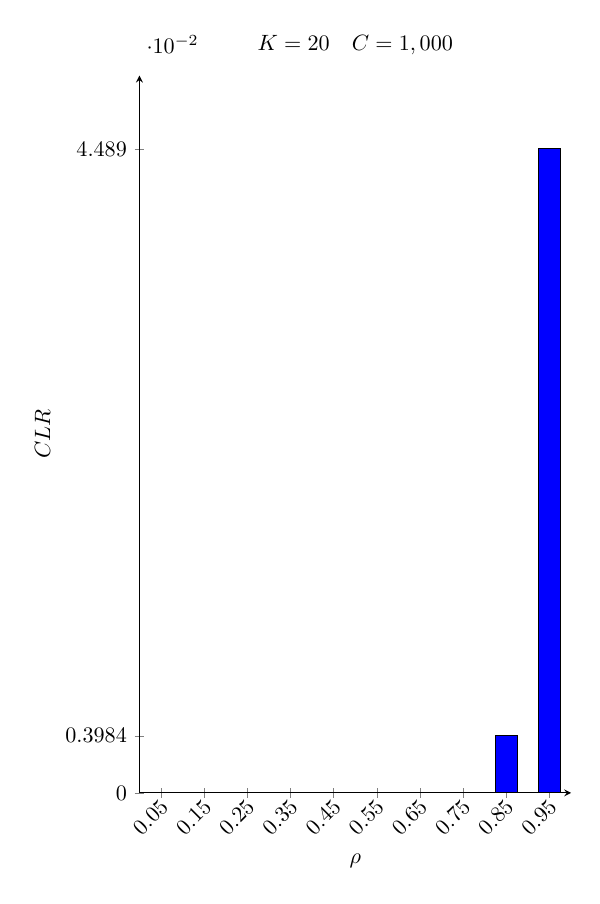
\begin{tikzpicture}[scale=0.8]
\begin{axis}[
    title= {$K=20 \quad C=1,000$},  
	ymin=0,
	ymax=.05,
	y post scale=2,
    ybar,
    xmin=0,
    xmax=1,
	xlabel = {$\rho$},
    ylabel = {$CLR$},
	xtick=data,
	ytick=data,
	ticklabel style={
        /pgf/number format/fixed,
        /pgf/number format/precision=5
	},
	x tick label style={rotate=45, anchor=east, align=center, xshift=.1cm,yshift=-0.1cm},
	axis lines=left
	]
\addplot [fill=blue] 
  coordinates
{(.05,.0) (0.15,.0) (0.25,.0) (0.35,.0) (0.45,.0) (0.55,.0) (0.65,.0) (0.75,.0) (0.85,.003984) (0.95,.044890) }
\closedcycle;
\end{axis}
\end{tikzpicture}
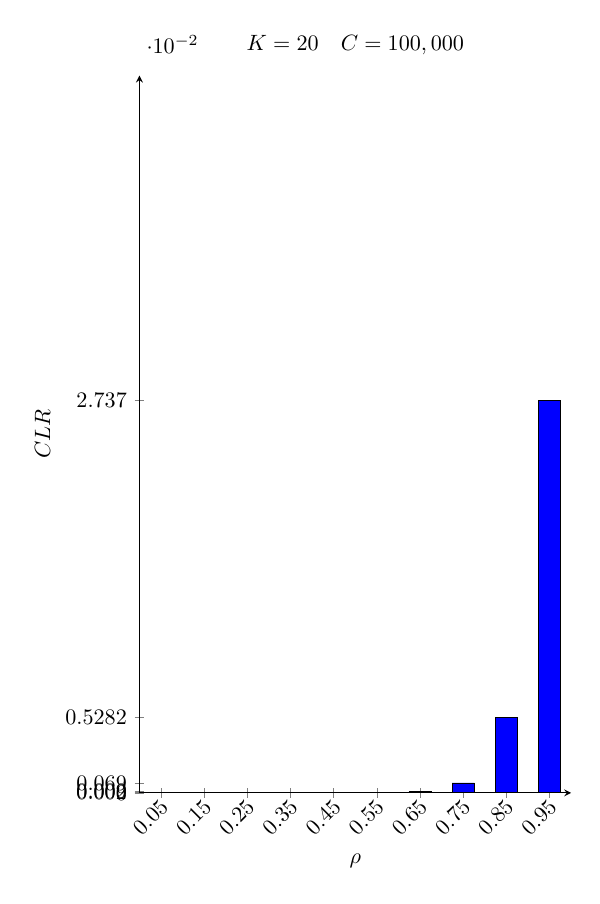
\begin{tikzpicture}[scale=0.8]
\begin{axis}[
    title= {$K=20 \quad C=100,000$},  
	ymin=0,
	ymax=.05,
	y post scale=2,
    ybar,
    xmin=0,
    xmax=1,
	xlabel = {$\rho$},
    ylabel = {$CLR$},
	xtick=data,
	ytick=data,
	ticklabel style={
        /pgf/number format/fixed,
        /pgf/number format/precision=5
	},
	x tick label style={rotate=45, anchor=east, align=center, xshift=.1cm,yshift=-0.1cm},
	axis lines=left
	]
\addplot [fill=blue] 
  coordinates
{(.05,.0) (0.15,.0) (0.25,.0) (0.35,.0) (0.45,.0) (0.55,0.000020) (0.65,0.000090) (0.75,.000690) (0.85,.005282) (0.95,0.027370)}
\closedcycle;
\end{axis}
\end{tikzpicture}
\\
For a constant queue capacity and completion size, where the queue capacity is large relative to the average number of customers in the system, the CLR increases quickly at higher values of $\rho$. Since the CLR represents the expected number of rejected requests ($E[reject]$), this number can be expected to remain close to 0 for large values of K and small values $\rho$.
}
\bigskip
\newpage


\textbf{Task 2}
Now let us fix $\rho = 0.85$. Plot the CLR against the value of the queue capacity $K$, as $K$ increases
from 10 to 100 in increments of 10. Again, submit two graphs: one for $C = 1,000$ and one for $C = 100,000$.
Explain the behavior of the plots as K increases, and especially, the rate of change in the CLR as a function
of K. Is this expected? Also, explain any differences in the two graphs due to the length of each simulation
run
\\
\medskip\\\texttt{
\\
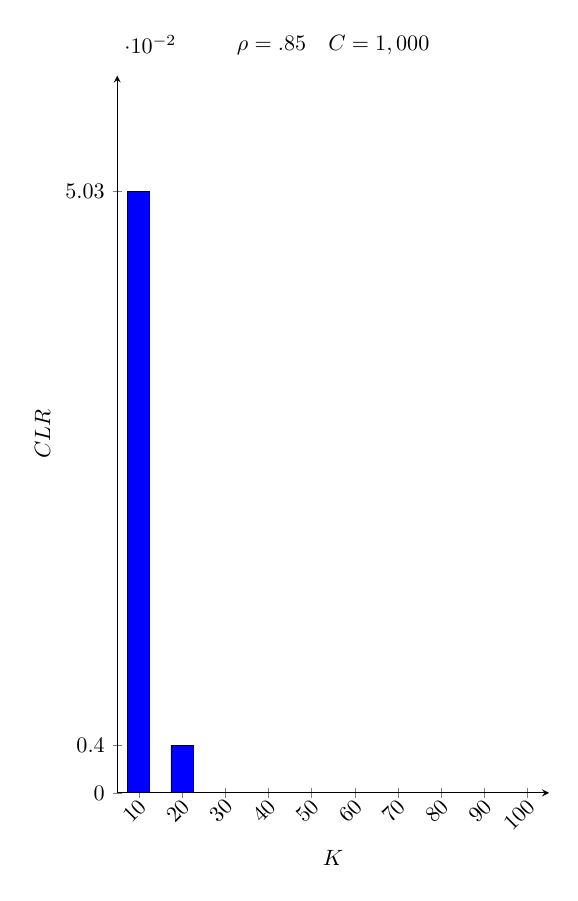
\begin{tikzpicture}[scale=0.8]
\begin{axis}[
    title= {$\rho=.85 \quad C=1,000$},  
	ymin=0,
	ymax=.06,
	y post scale=2,
    ybar,
    xmin=5,
    xmax=105,
	xlabel = {$K$},
    ylabel = {$CLR$},
	xtick=data,
	ytick=data,
	ticklabel style={
        /pgf/number format/fixed,
        /pgf/number format/precision=5
	},
	x tick label style={rotate=45, anchor=east, align=center, xshift=.1cm,yshift=-0.1cm},
	axis lines=left
	]
\addplot [fill=blue] 
  coordinates
{(10,.0503) (20,0.0040) (30,0) (40,0) (50,0) (60,0) (70,0) (80,0) (90,0) (100,0) }
\closedcycle;
\end{axis}
\end{tikzpicture}
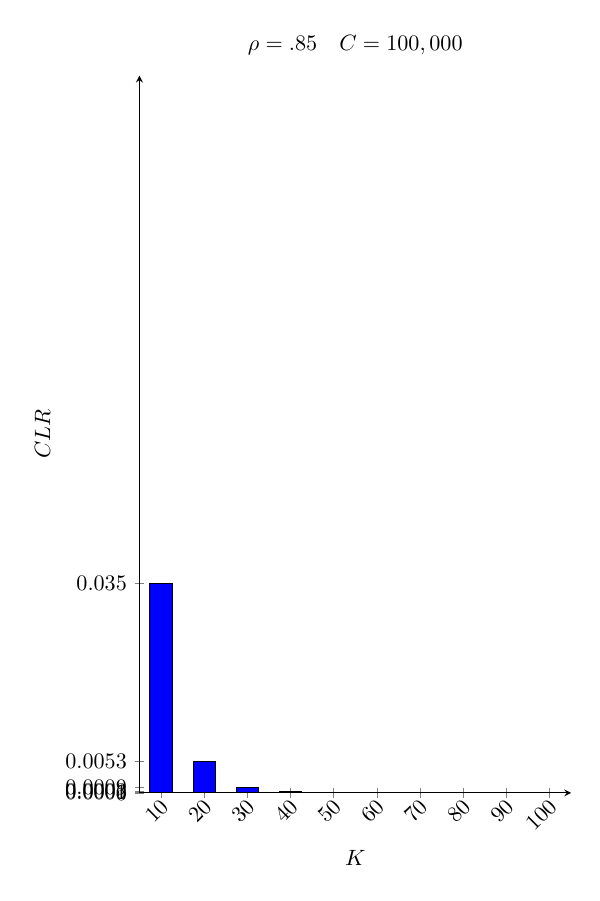
\begin{tikzpicture}[scale=0.8]
\begin{axis}[
    title= {$\rho=.85 \quad C=100,000$},  
	ymin=0,
	ymax=.12,
	y post scale=2,
    ybar,
    xmin=5,
    xmax=105,
	xlabel = {$K$},
    ylabel = {$CLR$},
	xtick=data,
	ytick=data,
	ticklabel style={
        /pgf/number format/fixed,
        /pgf/number format/precision=5
	},
	x tick label style={rotate=45, anchor=east, align=center, xshift=.1cm,yshift=-0.1cm},
	axis lines=left
	]
\addplot [fill=blue] 
  coordinates
{(10,.0350) (20,.0053) (30,0.0009) (40,0.0003) (50,0.0001) (60,0) (70,0) (80,0) (90,0) (100,0) }
\closedcycle;
\end{axis}
\end{tikzpicture}
\\
As $K$ increases, CLR approaches 0. This is because for larger values of $K$, there is less liklihood of a rejection. For larger values of $C$, there is a slower approach towards 0 due to the higher number of events that could result in a reject. This is expected.
}

\bigskip
\pagebreak

\textbf{Task 3}
The M/M/1/K system you simulate has an analytical solution for the CLR, which is given by:

\begin{equation}
  CLR=\frac{(1-\rho)\rho^K}{1-\rho^{K+1}}
\end{equation}

Let $K = 20$. For $C = 100,000$ and for $\rho = 0.05,\cdots, 0.95$ (in increments of 0.10), plot the simulation and analytical values of CLR on the same graph. Compare the simulation to the analytical values: are they
identical, close to each other, or completely different? What about the overall behavior of the curves as a
function of $\rho$? Explain
\\
\medskip\\\texttt{
\\
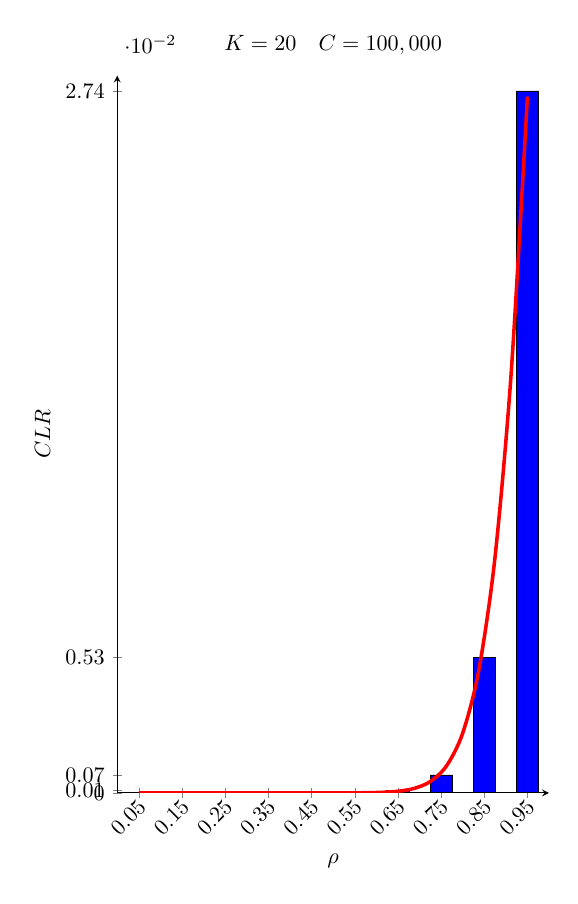
\begin{tikzpicture}[scale=0.8]
\begin{axis}[
    title= {$K=20 \quad C=100,000$},  
	ymin=0,
	ymax=.028,
	y post scale=2,
    ybar,
    xmin=0,
    xmax=1,
	xlabel = {$\rho$},
    ylabel = {$CLR$},
	xtick=data,
	ytick=data,
	ticklabel style={
        /pgf/number format/fixed,
        /pgf/number format/precision=5
	},
	x tick label style={rotate=45, anchor=east, align=center, xshift=.1cm,yshift=-0.1cm},
	axis lines=left
	]
\addplot [fill=blue] 
  coordinates
{(.05,0) (0.15,0) (0.25,0) (0.35,0) (0.45,0) (0.55,0) (0.65,0.0001) (0.75,0.0007) (0.85,0.0053) (0.95,0.0274)}
\closedcycle;
\addplot[color=red, smooth, ultra thick, domain=.05:.95]{((1-x)*x^20)/(1-x^(21))};
\end{axis}
\end{tikzpicture}
\\
As $\rho$ increases, the empirical and analytical values for CLR increase closely (within 10\%) of each other. The values increase rapidly for higher values of $\rho$, since the CLR value quickly approaches a limit defined as
$$\lim_{\rho \to 1} \frac{(1-\rho)\rho^K}{1-\rho^{K+1}} = \frac{1}{K+1}$$
In other words, the CLR limit is defined only by $K$. For $K=20$ the limit is $1/21 = 0.0476$.
}

\bigskip
\pagebreak

\textbf{Task 4}
Let us set $K = 100$ and $C = 100,000$. Compute the average waiting time $\overline{W}$ of the $C$ customers that have received service at the end of the simulation (i.e., ignore any lost customers or customers waiting
in the queue when the simulation ends). Plot $\overline{W}$ against the value of $\rho$ for $\rho = 0.05,\cdots, 0.95$. Is the result what you expected to see? Explain.
\\
\medskip\\\texttt{
\\
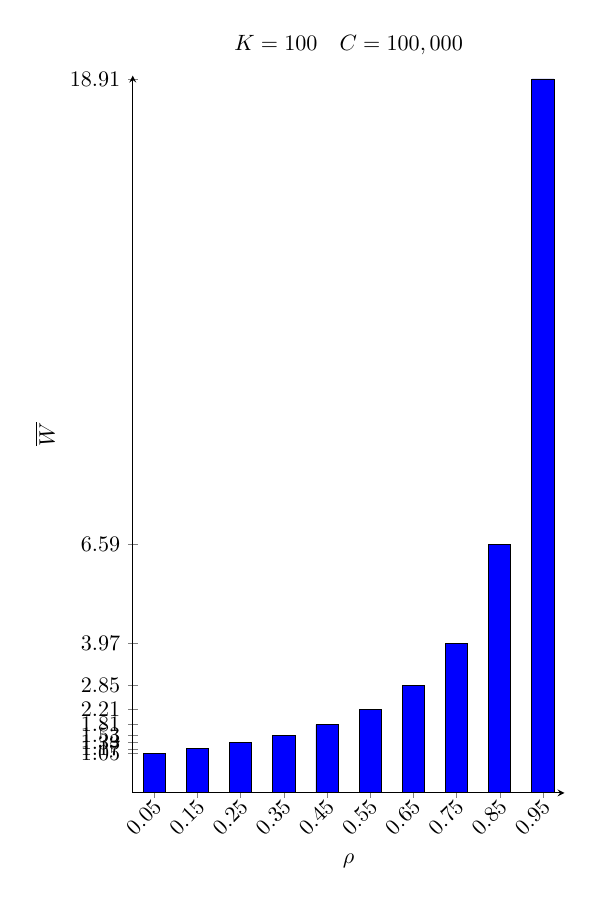
\begin{tikzpicture}[scale=0.8]
\begin{axis}[
    title= {$K=100 \quad C=100,000$},  
	ymin=0,
	ymax=19,
	y post scale=2,
    ybar,
    xmin=0,
    xmax=1,
	xlabel = {$\rho$},
    ylabel = {$\overline{W}$},
	xtick=data,
	ytick=data,
	ticklabel style={
        /pgf/number format/fixed,
        /pgf/number format/precision=5
	},
	x tick label style={rotate=45, anchor=east, align=center, xshift=.1cm,yshift=-0.1cm},
	axis lines=left
	]
\addplot [fill=blue] 
  coordinates
{(.05,1.05) (0.15,1.17) (0.25,1.33) (0.35,1.53) (0.45,1.81) (0.55,2.21) (0.65,2.85) (0.75,3.97) (0.85,6.59) (0.95,18.91)}
\closedcycle;
\end{axis}
\end{tikzpicture}
\\
As $\rho$ increases, the empirical values for $\overline{W}$ increase, which is expected since the wait times are dependent on the queue size at arrival, which will be longer for higher arrival rates. The value of $\overline{W}$ approaches $\frac{K}{2}$. This is expected.
}

\bigskip
\pagebreak

\textbf{Task 5}
Let us again set $K = 40$ and $C = 100,000$. Time the running time of your simulation for $\rho = 0.05,\cdots, 0.95$. Plot the running time against the value of $\rho$: is the running time increasing, decreasing, or constant as $\rho$ increases? Can you explain this behavior? Did you expect these results before running the
experiment?
\\
\medskip\\\texttt{
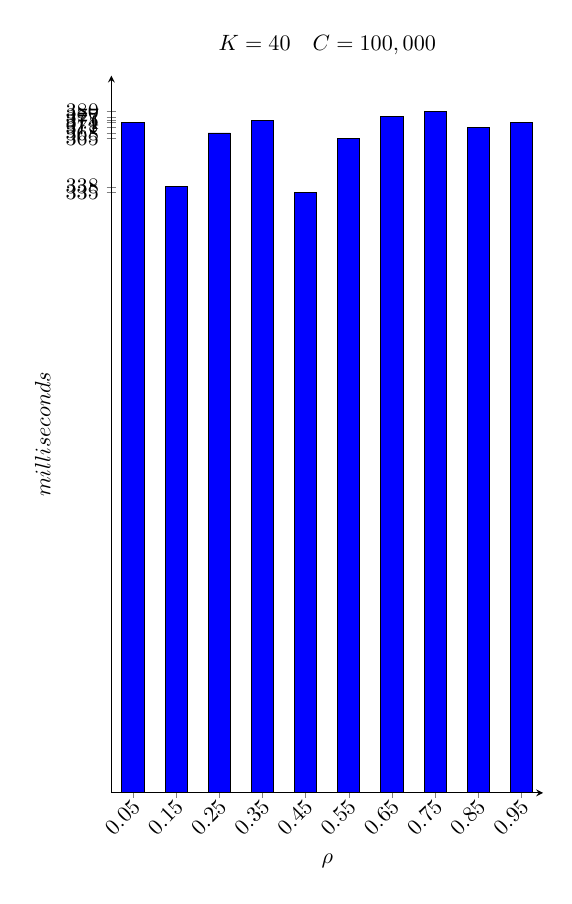
\begin{tikzpicture}[scale=0.8]
\begin{axis}[
    title= {$K=40 \quad C=100,000$},  
	ymin=0,
	ymax=400,
	y post scale=2,
    ybar,
    xmin=0,
    xmax=1,
	xlabel = {$\rho$},
    ylabel = {$milliseconds$},
	xtick=data,
	ytick=data,
	ticklabel style={
        /pgf/number format/fixed,
        /pgf/number format/precision=5
	},
	x tick label style={rotate=45, anchor=east, align=center, xshift=.1cm,yshift=-0.1cm},
	axis lines=left
	]
\addplot [fill=blue] 
  coordinates
{(.05,374) (0.15,338) (0.25,368) (0.35,375) (0.45,335) (0.55,365) (0.65,377) (0.75,380) (0.85,371) (0.95,374)}
\closedcycle;
\end{axis}
\end{tikzpicture}
\\
Because this simulator uses event times to increment the clock, the run times are near constant for values of $\rho$. However, for simulation values that produce a large number of rejects, the times do increase due to the number of rejects to process. This is expected.
}


\bigskip
\pagebreak

\textbf{Task 6}
Read the paper [Paxson96] of the reading list; this is an excellent example of a paper dealing with
measuring an existing system (in this case, the Internet). Answer (in less than one page) the following
questions:
\begin{enumerate}
\item What is "anticipatory flow state" and how is it related to routing asymmetry?
\\\\\texttt{Anticipatory flow state describes the scenario of router observing traffic from $A\rightarrow B$ and using this information to prepare for traffic from $B\rightarrow A$. This inference assumes that routing is roughly symmetrical (e.g., that  $A\rightarrow B$ implies $B\rightarrow A$) and if that expectation does not hold, then anticipatory flow states can create inefficient routing.}
\item What is "fluttering" and what are three problems that it creates?
\\\\\texttt{Fluttering describes rapidly-oscillating routing, where a return path or subsequent request takes a different route. The problems are
\begin{enumerate}
\item Unstable network paths. Unpredictable network routes are difficult to optimize and 
\item Asymmetric routing (see (a))
\item Metrics calculations are complicated by separate routes.
\end{enumerate}
}
\item Are routing pathologies getting better or worse in the Internet? What arguments does the author
provide for and against inferring trends from the data he presents?
\\\\\texttt{Given two data points in 1995, the authors cautiously suggest that pathologies are getting worse (increasing from 1.5\% to 3.4\%). There is a reason to suspect that 1995 was a red letter year due to the conversion of the NSFNET backbone to the commerically-operated backbone, but 1996 measurements seem to support the trend. Later papers by Paxson ("End-to-end Internet packet dynamics") repeat the finding, but show no continuing trend.}
\item Describe the organization of the paper. Is the structure what you would expect to see in a paper that
deals with measurements? Explain.
\\\\\texttt{The largest sections of the paper detail methodology (\S 4) and pathologies (\S 5). There is an unexpected detail on methodology limitations (\S 4.6). Also unexpected is the release for the raw data for reproducibility of the study. Unfortunately, this data is no longer available from the cited source, which is a common issue in older papers (see \url{http://dx.doi.org/10.1371/journal.pbio.1001745})}
\end{enumerate}


\bigskip



\label{last}
\end{document}

